\documentclass[spanish,12pt, a4paper, twoside]{paper}

\let\oldsection\section
\def\section{\cleardoublepage\oldsection}

\usepackage{afterpage}

\newcommand\blankpage{%
    \null
    \thispagestyle{empty}%
    \addtocounter{page}{-1}%
    \newpage}

\usepackage[textwidth=15cm, textheight=22.5cm, top=3.5cm, bottom=3.5cm,left= 4cm,right=2cm]{geometry}
\usepackage[spanish]{babel}
\usepackage{xeCJK}
\setCJKmainfont{DroidSansFallbackFull.ttf}
%\usepackage[applemac]{inputenc} 
%POR DEFECTO SE ESTÁ USANDO EL PAQUETE PARA RECONOCER ACENTOS DE MAC, EN CASO DE USAR WINDOWS COMO SISTEMA OPERATIVO ELIMINAR LA LÍNEA ANTERIOR E INTRODUCIR LA SIGUIENTE
\usepackage[utf8x]{inputenc}
\usepackage{libertine}

\usepackage{graphicx}
\usepackage{graphics}
\usepackage{amsmath,amssymb}
\usepackage{float}
\usepackage{changepage}
\usepackage{subcaption}
\usepackage{algorithm}
\usepackage{multirow}
\usepackage{hyperref}

\begin{document}
%\maketitle
%\thispagestyle{empty}
\begin{titlepage}

\newcommand{\HRule}{\rule{\linewidth}{0.5mm}} % Defines a new command for the horizontal lines, change thickness here

\center % Center everything on the page
 
%	HEADING SECTIONS

\includegraphics[width=4cm]{recursos/logoEtsisi.png}
  \hspace{8cm}

\includegraphics[width=2cm]{recursos/logo.png}
\\[1cm]

\textsc{\Large Escuela Técnica Superior de Sistemas Informáticos}\\[0.5cm]
\textsc{\large Universidad Politécnica de Madrid}
\\[3cm]


%	TITLE SECTION
 \HRule \\[0.4cm]
{ \huge \bfseries BFMB: Framework Base para Bots Modulares}\\[0.4cm] % Title of your document
\HRule \\[2.5cm]

\textsc{\LARGE Trabajo Fin de Grado}\\[0.5cm] 
\textsc{\Large Grado en Ingeniería del Software }\\[2.5cm]

 %	AUTHOR SECTION
\begin{flushright}
\large
AUTOR: Ángel González Abad\\
TUTOR: Dr. Francisco Javier Gil Rubio
\end{flushright}

\vspace{1.3cm}

%	DATE SECTION
{ {2018}}\\[3cm]
%	LOGO SECTION

\vfill % Fill the rest of the page with whitespace

\end{titlepage}

\afterpage{\blankpage}
\pagenumbering{roman}


%	AGRADECIMIENTOS
\section*{AGRADECIMIENTOS}
Aquí estarán los agradecimientos cuando se me ocurra que poner.

%	RESUMEN
\section*{RESUMEN}
Los chatbots no son aplicaciones que haya surgido recientemente, ya estuvieron presentes durante años en la investigación y en las redes con el desarrollo de Internet y la web. Pero es ahora cuando existe un ''boom'' en ellos, sobre todo gracias a los servicios que conforman la Web 2.0 y los recientes asistentes virtuales, tales como Siri, Alexa o Google Now.
\newline

El problema que surge a la hora de desarrollar un bot conversacional o una máquina de estados es cuando el desarrollador tiene como requisito la necesidad de interactuar con varios medios de forma simultánea. Por ejemplo, un sistema que requiera una comunicación simultánea entre redes sociales o un sistema que mande órdenes a un conjunto de dispositivos IoT (Internet of Things), ya que cada servicio utilizará protocolos e interfaces diferentes. Esto aumenta la complejidad en el desarrollo y puede producir duplicidades si se quieren desarrollar varios bots con usos diferentes.
\newline

Ante esta problemática, mi proyecto se basará en un sistema base para desarrollar bots (u otro tipo de automatismos software) multiprotocolo. Dicho sistema se compone de un servidor de comunicaciones central al que podemos anexar diferentes conectores que interactúan con los servicios de terceros. Cada conector pertenece a un servicio concreto, donde podremos activar los que nos sean útiles. La parte lógica del bot se comunica con el servidor a través de JSON-RPC sobre HTTP, HTTPS, TLS sobre TCP o TCP (dependiendo de las necesidades del proyecto).
\newline

La finalidad de este proyecto es hacer que el desarrollador se centre en la lógica y en la inteligencia que pueda tener en mayor o menor nivel en lugar de tener que centrarse en las interfaces de los servicios de terceros.


%	SUMMARY
\section*{SUMMARY}
Extensión máxima de una página

%	ÍNDICE
\tableofcontents % indice de contenidos

%	INDICE DE FIGURAS Y TABLAS
\listoffigures
\listoftables

%	CAPÍTULOS DEL TRABAJO FIN DE MÁSTER
\newpage
\pagenumbering{arabic} 

\section{INTRODUCCIÓN Y OBJETIVOS}

Los chatbots no son aplicaciones que hayan surgido recientemente, sino que han tenido una larga historia por detrás. Desde el primer software chatbot (ELIZA en 1966), se han realizado desarrollos de chatbots hasta la actualidad. Pero es ahora cuando existe cierto surgir comercial de estos, gracias sobre todo a los asistentes virtuales de las grandes empresas tecnológicas como Siri, Alexa, Watson o Google Now.
\newline

Pero existe una problemática para quienes quieran realizar un chatbot: la necesidad de una conexión con el exterior para poder comunicarse. No suele ser compleja esta parte si solamente va a interactuar con un único servicio, pero cuando se requiere la conexión a múltiples servicios e interactuar con ellos de forma simultánea, la complejidad del desarrollo aumenta, llegando a dedicar más recursos a la conexión de servicios que a la lógica del software.
\newline

Para ello nace la idea propuesta para este proyecto final de grado. Me centraré en el desarrollo de un sistema base por el cual nuestro nuevo bot se conectará a los servicios que requiera. No solo valdría para chatbots y su conexión a redes de chat o redes sociales, sino también para máquinas de estados conectadas a servicios IoT. Este sistema se centra en las comunicaciones para que el desarrollador solamente tenga que centrarse en desarrollar la lógica, el cual ya supone bastante trabajo.
\newline

Este proyecto cubre los siguientes objetivos:

\begin{itemize}
\item El desarrollo de un servidor de comunicaciones que hará de mediador entre el bot y los servicios externos en Internet, usando para ello unos módulos denominados conectores.
\item La creación de uno o dos de esos módulos conectores para interactuar con los servicios de terceros.
\item La creación de un bot sencillo para poder realizar las demostraciones de funcionamiento.
\end{itemize}

\section{ESTADO DEL ARTE}

\subsection{Historia de los chatbots}

\subsubsection{Origen}

El origen del nombre ''chatbot'' viene de un software llamado CHATTERBOT, el cual era un jugador virtual del videojuego de mazmorras TinyMUD. La principal tarea de este bot era responder a las preguntas de los usuarios que tenían relación con la navegación por la mazmorra u objetos del juego. El mismo simulaba habilidad conversacional mediante reglas, mediante las cuales logró ''engañar'' a los usuarios y que estos creyeran que era un jugador humano más. \cite[pág. 2]{CANLI}

\subsubsection{ELIZA}
ELIZA fue un programa de procesamiento del lenguaje natural creado entre los años 1964 y 1966 por Joseph Weizenbaum (1923-2008) en el Laboratorio de Inteligencia Artifical del MIT (Instituto Tecnológico de Massachusetts). El objetivo de este software era demostrar la superficialidad de la comunicación entre humanos y máquinas.
\newline

El software que realizó fue una de las primeras vías de interacción entre persona y máquina mediante el uso del lenguaje natural. El mismo era una parodia de un terapéuta que ejercía psicoterapia centrada en el cliente, una teoría psicológica creada por el psicólogo norteamericano Carl Rogers. El software reutilizaba con frecuencia las frases enviadas por el cliente y las convertía en preguntas para el mismo.
\newline

ELIZA era un \emph{software} limitado, ya que solo fue programado para responder a ciertas palabras o frases clave. Así que lo normal era llegar a conversaciones sin sentido.

\subsubsection{Actualidad: Asistentes virtuales}

\section{ANÁLISIS}

\subsection{Idea base del proyecto}

La idea principal es el desarrollo de un sistema de comunicaciones con diversas APIs externas para facilitar el desarrollo de bots o automatismos que interactúen con ellos. En sí no forma una aplicación, sino que será una base para que otras personas puedan realizar sus aplicaciones. Por ello, es un framework.
\newline

Un framework es un software compuesto de componentes personalizables e intercambiables para el desarrollo de una aplicación. Podría considerarse como una aplicación genérica incompleta en donde se añadan las últimas piezas. \cite[pág. 1]{FrameworkJJG}

\subsection{Tecnologías usadas}

\subsubsection{JSON-RPC}

JSON-RPC es un protocolo de llamada a procedimiento remoto (Remote Procedure Cell) cliente-servidor cuyos mensajes se componen de datos codificados en formato JSON (Javascript Object Notation). Es un protocolo agnóstico, por lo que puede realizar comunicaciones cliente-servidor a través de HTTP, HTTPS o TCP, entre otros. La especificación más reciente es la versión 2.0, publicada en 2010.

Como el protocolo usa JSON como mensaje, dispone de las mismas características que un fichero JSON: dispone de los cuatros tipos primitivos (String, Number, Boolean y Null) y de dos tipos de estructura (Object y Array).
El protocolo en sí se basa en dos modelos de datos: petición (Request) y respuesta (Response), los cuales explico a continuación:

\begin{itemize}
\item \textbf{Objeto petición (Request):} La llamada a procedimiento remoto en JSON-RPC se basa en enviar este objeto a un servidor, el cual dispone de los siguientes atributos:

\begin{itemize}
\item \textbf{jsonrpc:} Atributo que especifica la versión del protocolo JSON-RPC. Debe ser "2.0" para la versión 2.0 y cambia según el número de versión.

\item \textbf{method:} Un String donde se indica el método a invocar. Cualquier nombre de método es válido excepto los que empiecen con "rpc.", ya que son de uso interno.

\item \textbf{params:} Un atributo de tipo estructura que indica los parámetros a enviar al método. Es un atributo que puede ser opcional.

\item \textbf{id:} Un identificador establecido por el cliente que puede ser un tipo distinto de Boolean (y Null, en base a las actualizaciones de la especificación). Si este valor no está includo, el protocolo considera la petición como una notificación.
\end{itemize}

\item \textbf{Objeto respuesta (Response):} La llamada a procedimiento remoto en JSON-RPC debe devolver una respuesta a cada petición excepto si es una notificación. El objeto respuesta tiene los siguientes atributos:

\begin{itemize}
\item \textbf{jsonrpc:} Atributo que especifica la versión del protocolo JSON-RPC. Debe ser "2.0" para la versión 2.0 y cambia según el número de versión.

\item \textbf{result:} Este atributo es obligatorio si el resultado es exitoso y, en caso contrario (error), no debe estar presente. Siempre va a ser un atributo de estructura.

\item \textbf{error:} Este atributo debe existir en los casos de error y no aparecer en casos de éxito. Siempre va a ser un atributo de estructura.

\item \textbf{id:} El identificador en las respuestas es obligatorio y debe ser el mismo id que el recibido en el objeto de la petición. En caso de no llegar un id correcto, el valor de este atributo debe ser Null.
\end{itemize}

\item \textbf{Objeto error:} Si una llamada a procedimiento remoto encuentra un error, el objeto respuesta debe incorporar este objeto de error en el atributo denominado como tal. El objeto error tiene los siguientes atributos:

\begin{itemize}
\item \textbf{code:} Código de error de JSON-RPC

\item \textbf{message:} Un String que indica la descripción resumida del error.

\item \textbf{data:} Atributo de tipo primitivo o de estructura que entrega información adicional del error. Es un atributo opcional.
\end{itemize}

\end{itemize}

\subsection{Servicios utilizados}

\subsubsection{Tadoº}

Tadoº GmbH es una empresa tecnológica alemana con sede en Múnich y es un fabricante de sistemas de automatización de calefacción y refrigeración para el hogar conectados a Internet.
\newline

Fundado en el año 2011 por Johannes Schwarz, Christian Deilmann y Valentin Sawadski, el nombre de dicha compañía está inspirado en una unión de las expresiones japonesas ''tadaima'' (ただいま), que significa ''Estoy en casa'' y ''okaeri'' (おかえり), que significa ''Bienvenido'' a la hora de dirigirse a alguien con quien convives. Puede parecer que la presencia de este párrafo no tenga mucho sentido pero lo tiene, ya que uno de los valores añadidos de sus sistemas de automatización es, precisamente, la gestión de la climatización basándose en la geolocalización.
\newline

Su gestión basada en geolocalización se realiza de la siguiente forma: El usuario o usuarios de la vivienda tienen asociado un dispositivo móvil, el cual debe tener la app de la compañía instalada y configurada. Esta app recoge la posición actual y se compara con un \emph{geofence} \footnote{El término \emph{geofence} es un perímetro virtual asociado a un área geográfica. Su utilidad se basa en la ejecución de eventos en software ante un suceso de entrada o salida del área definida. } definido por el usuario maestro de la vivienda. Cuando todos los usuarios de la vivienda abandonan la zona definida por el \emph{geofence}, Tado ordena la desconexión de la calefacción o la reducción de la temperatura de las estancias.
\newline

Otra de sus funcionalidades es la detección de ventanas abiertas. Los sensores instalados (termostatos y válvulas) detectan la temperatura y en la humedad, y los cambios repentinos en los mismos se asocian con la apertura de ventanas. Ante ello, Tado desconecta la calefacción por un tiempo definido en la configuración (entre 5 y 45 minutos) para evitar el consumo innecesario de energía.
\newline

La última funcionalidad adicional que provee es el ajuste de potencia en la calefacción basándose en el tiempo atmosférico actual. La calefacción se ajusta en base a la estimación de incidencia solar que puede haber.

\paragraph{Dispositivos}

Tadoº, en sus sistemas de calefacción, tiene distintos dispositivos de gestión, los cuales explico a continuación:

\begin{itemize}
\item\textbf{Puente de conexión (Bridge):} Es el dispositivo de conexión entre Internet (la api de Tado) y la red 6LoWPAN\footnote{6LoWPAN (IPv6 over Low-Power Wireless Personal Area Networks) es un estándar que adapta la transmisión de paquetes IPv6 a redes que siguen el estándar IEEE 802.15.4, los cuales son dispositivos con recursos muy limitados y un flujo de datos muy bajo. Otra característica de esta red es la capacidad de crear redes en malla.} en la que se comunican los dispositivos entre sí. Funciona con una conexión Ethernet y una conexión USB para alimentación eléctrica.

\item\textbf{Termostato:} Dispositivo que tiene la capacidad de encender o apagar la caldera o ajustar su potencia (según compatibilidad de calderas). Para ello, dispone de un relé para la conmutación. Incluye sensores para la medida de temperatura y humedad. Funcionan con tres pilas AAA y pueden ser instalados también como controladores de temperatura inalámbricos.

\item\textbf{Válvula termostática:} Mecanismo eléctrico que incluye sensores para la medición de temperatura y humedad. Con ellos, activa un motor que regula la apertura de la válvula del radiador donde se encuentre instalado y también pueden regularse de forma manual. Funcionan con dos pilas AA.
\end{itemize}

Pueden ver las fotografías de cada dispositivo en la figura ~\ref{fig:aparatos tado}.

\begin{figure}[htp]
\begin{subfigure}{0.5\textwidth}
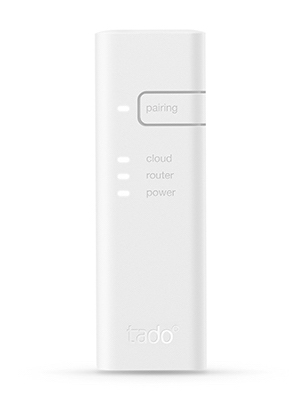
\includegraphics[width=\textwidth]{recursos/bridge.jpg}
\caption{Puente de conexión}
\label{fig:bridge tado}
\end{subfigure}
\begin{subfigure}{0.5\textwidth}
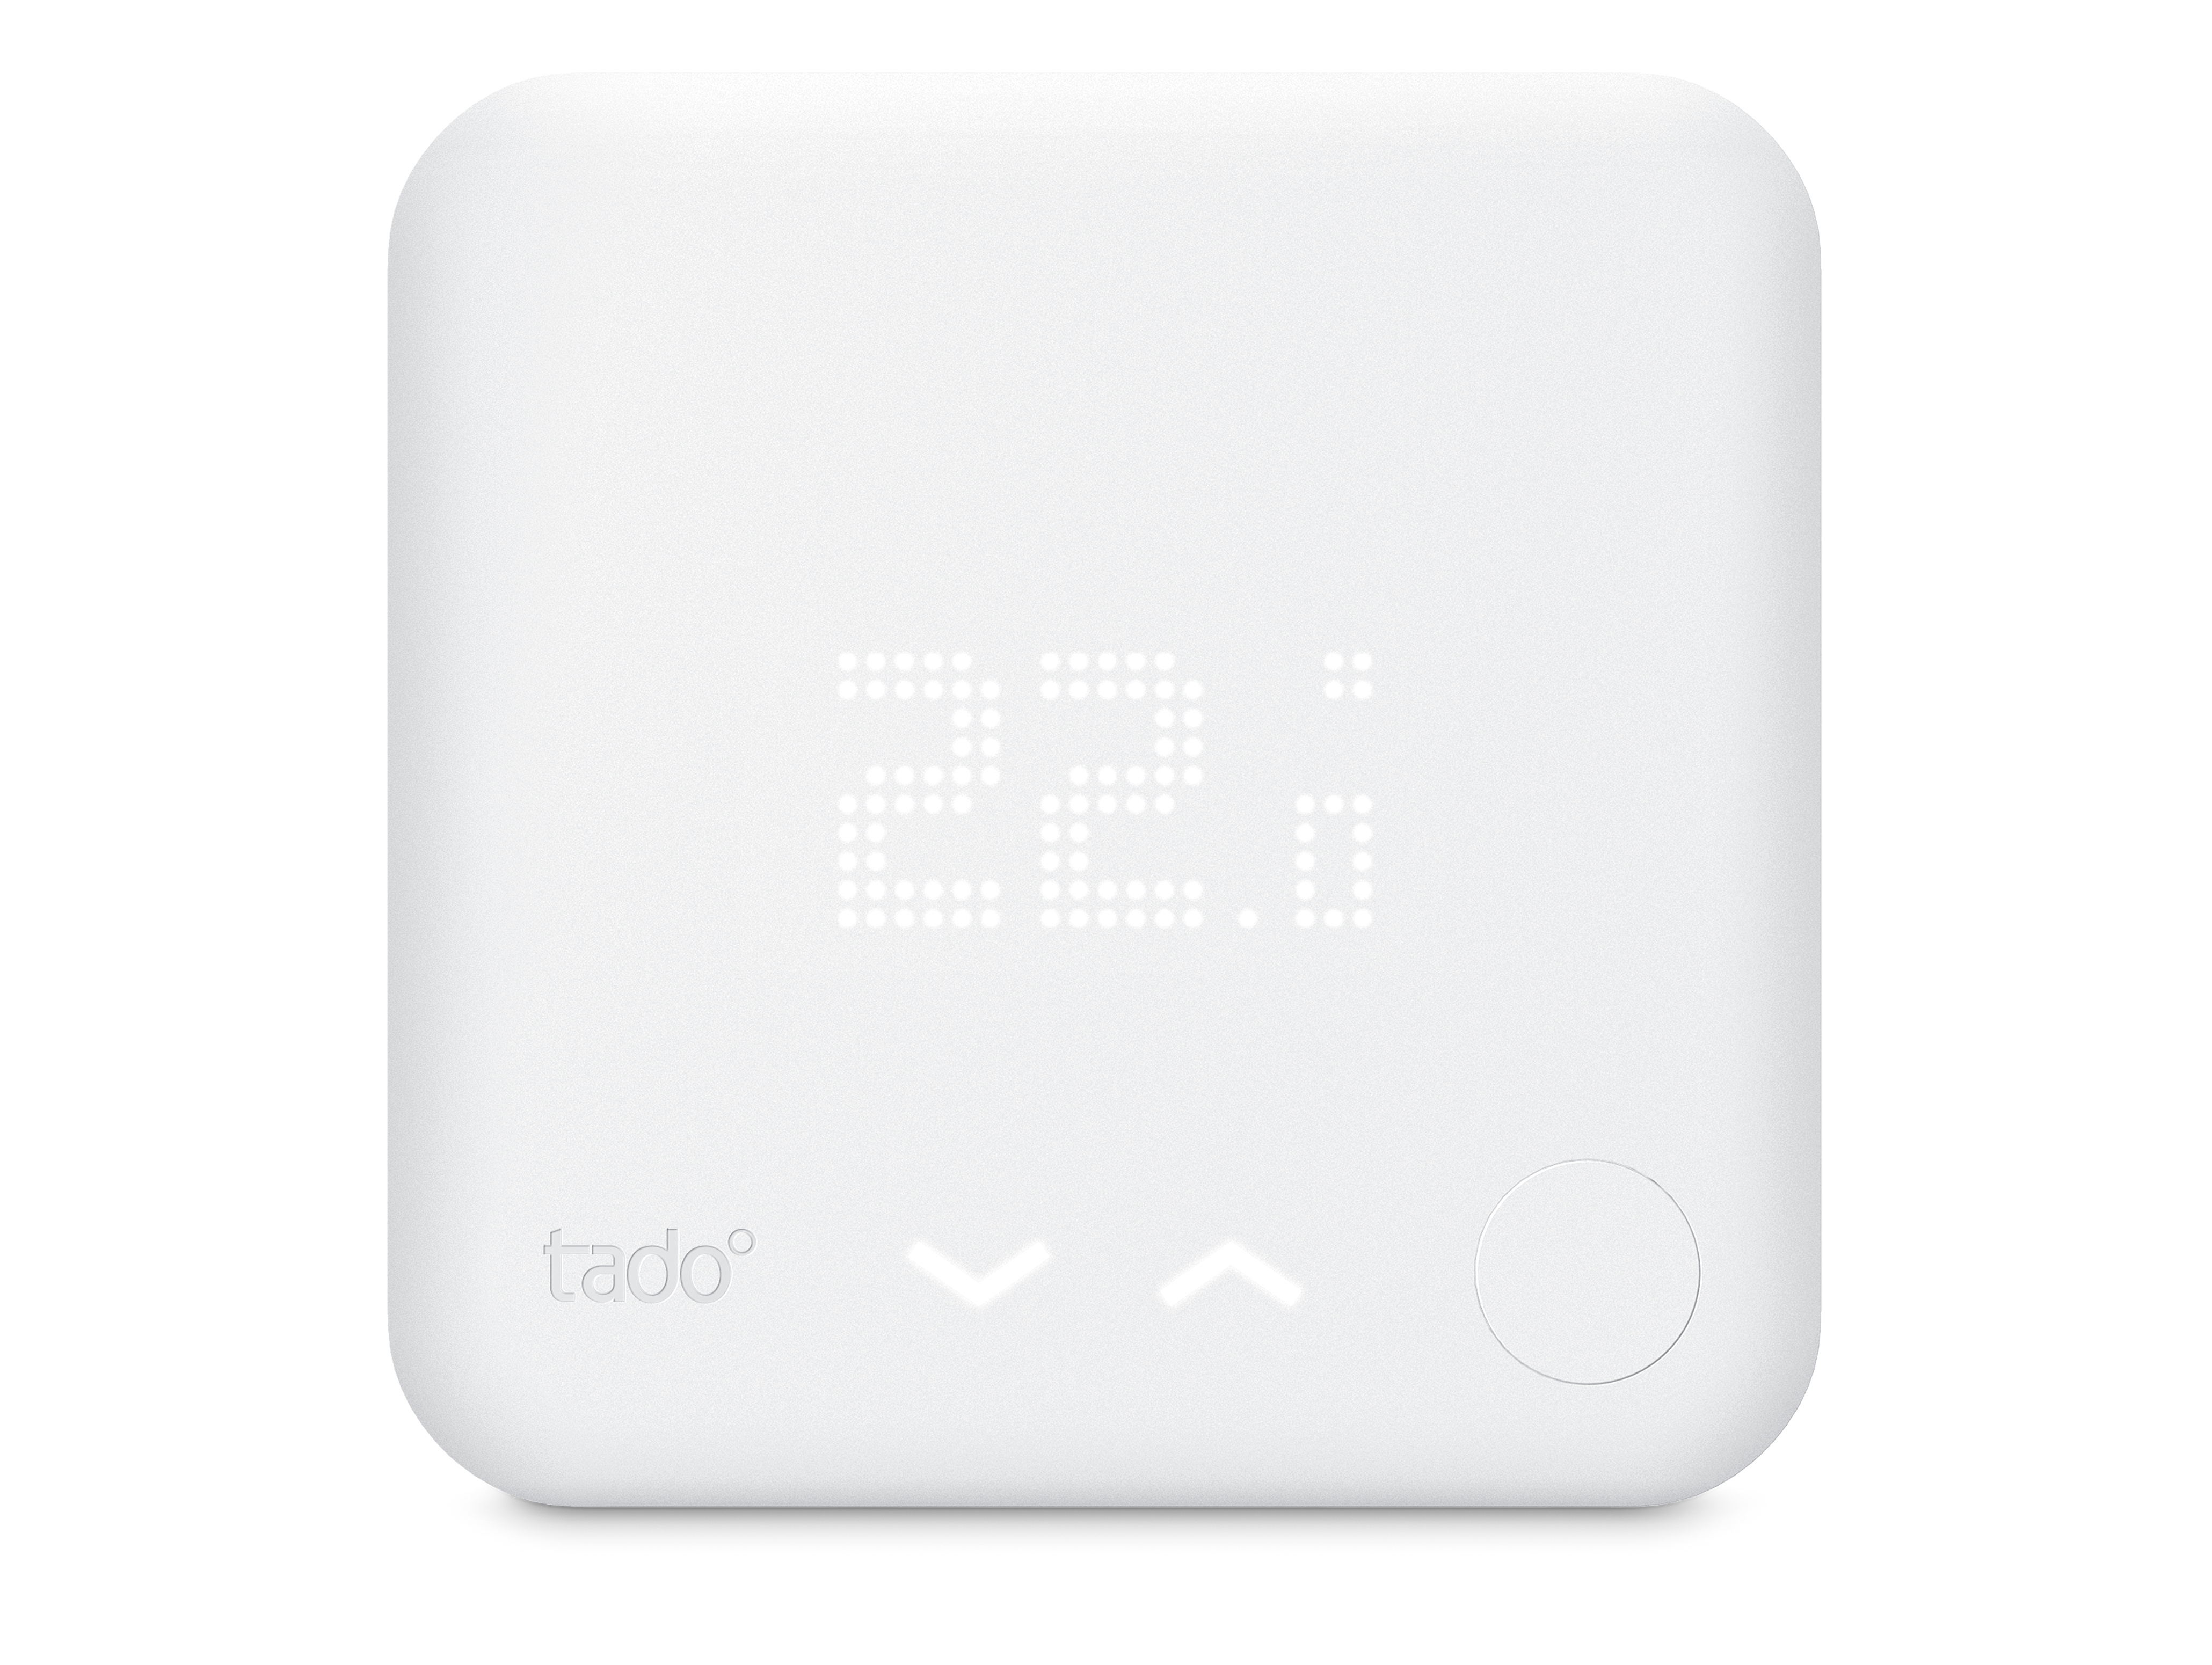
\includegraphics[width=\textwidth]{recursos/termostato.jpeg}
\caption{Termostato Tadoº}
\label{fig:termostato tado}
\end{subfigure}
\begin{subfigure}{0.5\textwidth}
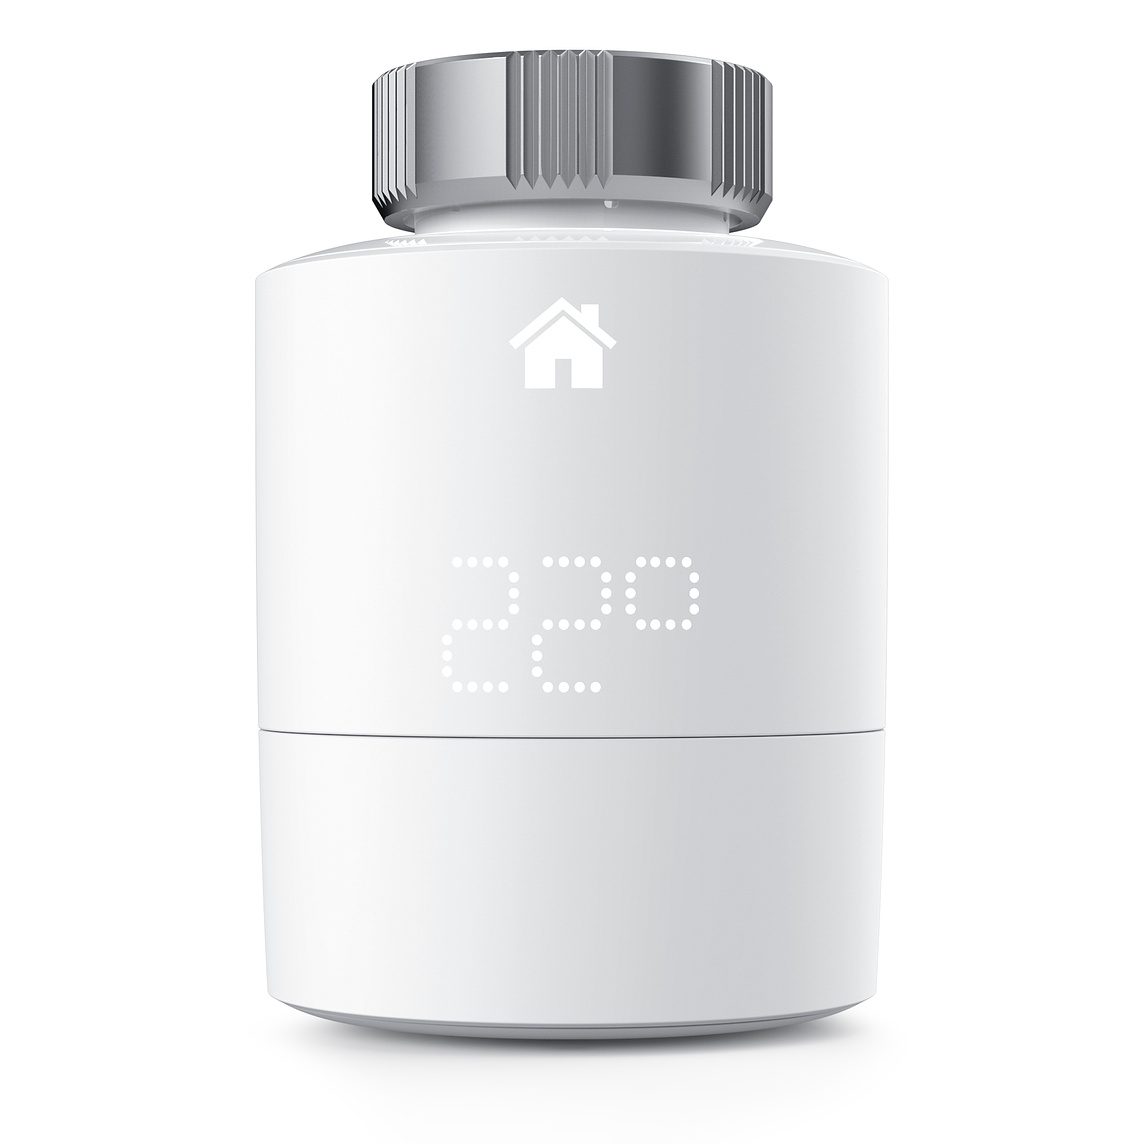
\includegraphics[width=\textwidth]{recursos/valvula.jpeg}
\caption{Válvula termostática Tadoº}
\label{fig:valvula tado}
\end{subfigure}

\caption{Aparatos de gestión de calefacción de la empresa Tadoº}
\label{fig:aparatos tado}
\end{figure}

\subsubsection{Telegram}

Telegram es un servicio de mensajería instantánea y VoIP\footnote{VoIP: Voz por protocolo de Internet. Permite la transmisión de la voz a través de Internet usando el protocolo IP. Se usa actualmente por los proveedores de telefonía en lugar de la telefonía analógica.} creado en el año 2013 por Nikolai y Pavel Durov, quienes anteriormente crearon la red social VK, conocida en Rusia. Se estima que el servicio tiene 200 millones de usuarios activos al mes.

Las funcionalidades que dispone el servicio son las siguientes:

\begin{itemize}
\item \textbf{Acceso multiplataforma:} Telegram, a diferencia de otras redes, permite que un usuario esté activo en varios dispositivos a la vez, sin obligar a cerrar la sesión del resto de conexiones ni borrar el contenido de los chats almacenados. Lo que sí requiere es registrar la cuenta de Telegram con un número de teléfono móvil.

\item \textbf{Capacidad para adjuntos de gran tamaño:} Gracias al protocolo MTProto, creado por Nikolai Durov, es posible transferir adjuntos multimedia de hasta 1,5GB de tamaño.

\item \textbf{Grupos y canales:} Para conversaciones entre varias partes, existe la creación de grupos. En ellos pueden haber hasta 200 000 usuarios y se pueden realizar respuestas a un mensaje concreto del chat, mencionar a un usuario y generar \emph{hashtags}\footnote{Cadena de caracteres que se usa para clasificar la información presente. Sería un tipo de metadato.}. Dichos grupos pueden ser públicos o privados y disponer de varios administradores.

Por otra parte, los canales están pensados para difusión de mensajes por parte de uno o varios administradores. No existe límite de usuarios en los canales, por lo que cualquiera puede acceder. Al igual que los grupos, los canales pueden ser públicos o privados y tienen las mismas capacidades (pueden enviar adjuntos y mensajes, aunque el resto de usuarios no puedan hacer uso de ello).

\item \textbf{Bots:} En Telegram es posible el uso de bots y se incentiva el desarrollo de nuevos bots gracias a la documentación que se provee a los desarrolladores. Los bots pueden ser configurados de distintas formas (escuchando comandos, escuchando menciones o cualquier mensaje). También existen los \emph{inline bots}, son bots que no requiren estar presentes en un chat para funcionar y proveen datos en base una consulta.

\item \textbf{Stickers:} Una extensión de los emojis para poder expresar reacciones de forma breve y visual. Los stickers ya eran una característica que ya tenía la aplicación de mensajería LINE, creada en 2011.

\item \textbf{Chats secretos:} Telegram provee la opción de usar chats secretos entre dos usuarios. Para ello, se utiliza cifrado extremo a extremo\footnote{El cifrado extremo a extremo (End-to-end encryption) es un sistema de comunicación donde dos usuarios pueden comunicarse sin que sus mensajes sean captados por los nodos intermedios en una red.} Por defecto, Telegram no activa este tipo de chats, ya que ciertas funcionalidades de Telegram no funcionan con este tipo de chats, como el acceso multiplataforma o los bots.

\item \textbf{VoIP:} Al igual que otros servicios de mensajería actuales, dispone de servicio de llamadas por voz. 

\item \textbf{Inicio de sesión en sitios terceros:} Telegram también tiene implementado un sistema para poder iniciar sesión con las credenciales del servicio en páginas web terceras, siempre que estas incluyan los componentes necesarios para ello. 

\end{itemize}

\section{DISEÑO Y ARQUITECTURA DEL SISTEMA}

\subsection{Metodología de trabajo}

\subsection{Casos de uso}

Los casos de uso para este proyecto están definidos a través de dos actores: el software que va a realizar las órdenes (el bot) y el usuario.

El bot realizará los siguientes casos de uso:

\begin{itemize}
\item El bot solicitará un autenticación con el servidor de comunicaciones (uno de los componentes del framework), el cual se envía un usuario y una contraseña al mismo. El servidor realiza la autenticación, comprobando si el usuario existe y si el hash de la contraseña guardada coincide con el hash generado de la contraseña enviada. Si la autenticación tiene éxito, se genera un token con los datos necesarios del usuario para poder realizar las acciones pertinentes.

\item El bot puede solicitar mensajes. Esta acción es una abstracción de las órdenes GET de una API HTTP REST. Para ello, antes de realizar acción alguna, se solicita el token que se recibió al autenticar para así validar la acción. Tras la verificación exitosa, se solicita los datos requeridos a través del servidor de comunicaciones. El servidor de comunicaciones dispone de unos componentes que denominaremos como "conectores", los cuales transforman la solicitud en los datos necesarios para el endpoint elegido. La respuesta o el error de la solicitud a la api la devuelve el servidor de comunicaciones.

\item El bot puede enviar mensajes. Esta acción es una abstracción de las órdenes POST, PUT y DELETE de una API HTTP REST. Al igual que con el caso de uso ya definido anteriormente, se verifica el token, se transforma el contenido y se envía a la api. La respuesta o error se devuelve a través del servidor de comunicaciones.
\end{itemize}

Por otra parte, el usuario realizará los siguientes casos de uso:

\begin{itemize}
\item A través de las aplicaciones que disponga cada servicio, el usuario interactúa con dichos servicios. Por ejemplo, puedo interactuar con el bot a través de un chat (Telegram) o cambiar la configuración de la calefacción (Tadoº).
\end{itemize}

\begin{figure*}
\centering
	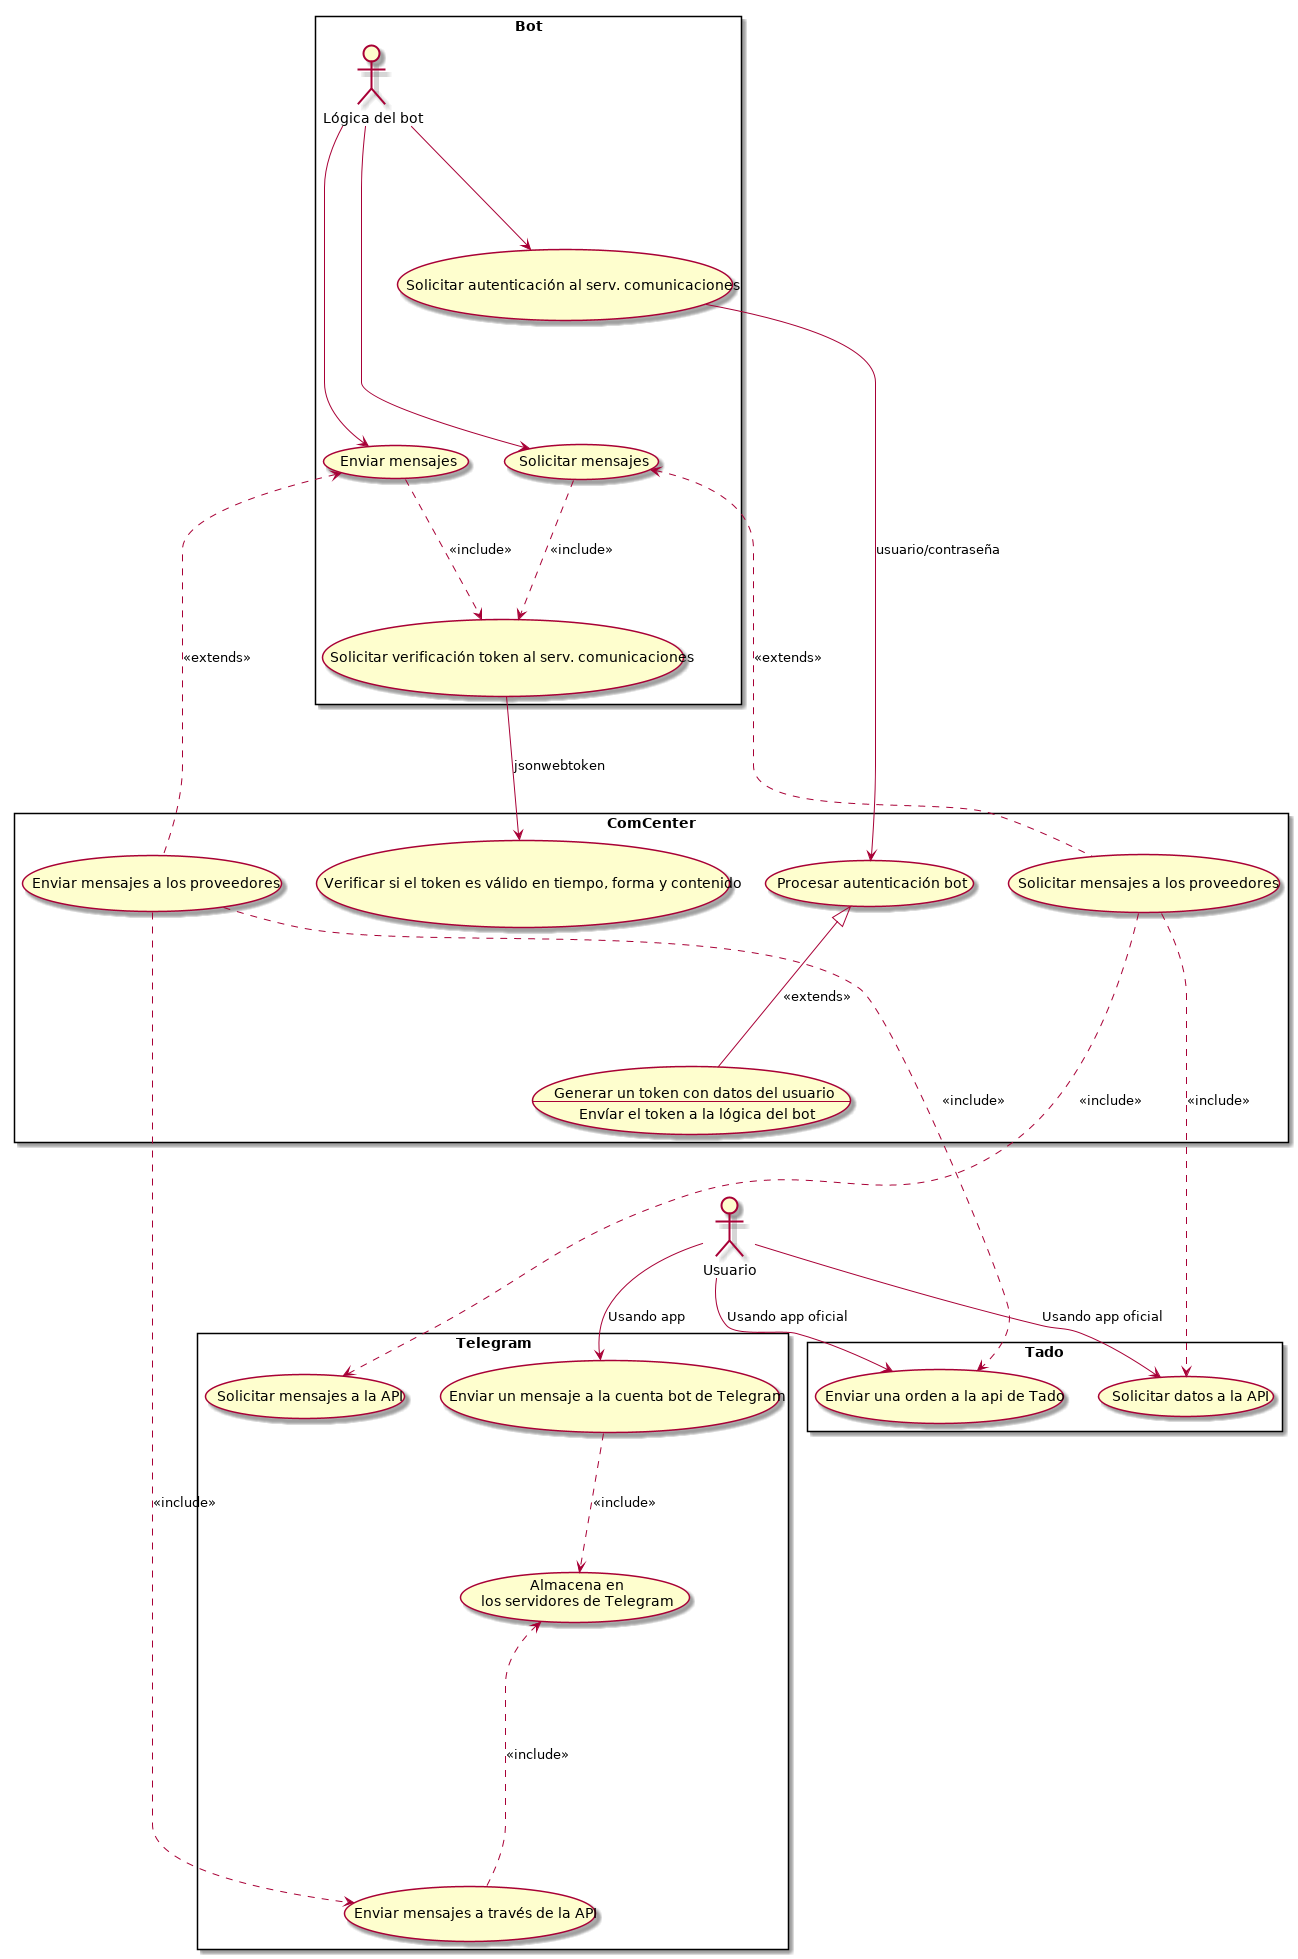
\includegraphics[width=\textwidth]{recursos/usecases}
\caption{Diagrama de casos de uso}
\label{fig:Diagrama de casos de uso}
\end{figure*}

\subsection{Infraestructura}

El framework BFMB requiere la ejecución de dos aplicaciones (el bot y el servidor de comunicaciones) y un servidor de Base de Datos (en este caso es MongoDB). Pueden ejecujarse en máquinas independientes o todo en una única máquina.
\newline

Ahora, vamos a definir en detalle cada aplicación:

\subsubsection{Software bot}

El software bot es la aplicación que realizará la persona que quiera utilizar este framework. Dicha aplicación puede desarrollarse en cualquier lenguaje de programación; el único requisito que debe tener para funcionar con este framework es la capacidad de poder usar el protocolo JSON-RPC, ya sea usando una biblioteca externa o una implementación propia.

\subsubsection{Servidor de comunicaciones}

El servidor de comunicaciones es una aplicación desarrollada en el lenguaje Typescript, el cual se compila a Javascript y se ejecuta usando NodeJS. Dicha aplicación contiene las siguientes funcionalidades:

\begin{itemize}
\item \textbf{Servidor JSON-RPC:} Usando una biblioteca externa llamada jayson, se ha realizado la implementación del servidor JSON-RPC. Lo único que hay que acoplar son los métodos que pueden ser accesibles a través del protocolo. Las aplicaciones bot pueden conectarse a través de protocolo TCP puro, TLS, HTTP o HTTPS. Para los protocolos seguros se requiere disponer de un certificado que pueda ser reconocido por una CA\footnote{Autoridad de certificación}, sea propia o externa.

\item \textbf{Conectores de servicio:} Los conectores son un elemento imprescindible para este software, son quienes permiten la conexión del servidor con los servicios externos a los que queramos acceder. Por el momento y para este proyecto, se han desarrollado dos conectores de servicio: uno para el servicio de mensajería instantánea Telegram y otro para un servicio que gestiona sistemas de calefacción IoT de la marca Tadoº. Son quienes realizan la conexión a la api usando los datos que se envían por parte del bot.

\item \textbf{Almacenamiento de credenciales:} Para garantizar que solo las aplicaciones autorizadas puedan usar el servidor de comunicaciones, se crean usuarios en una base de datos MongoDB. El detalle de los datos que se almacenan los mostraré en la siguiente sección pero, en resumen, el servidor almacena credenciales para acceder al servidor y los token y/o credenciales de las apis a las que debe acceder.
\end{itemize}

\begin{figure*}
\centering
	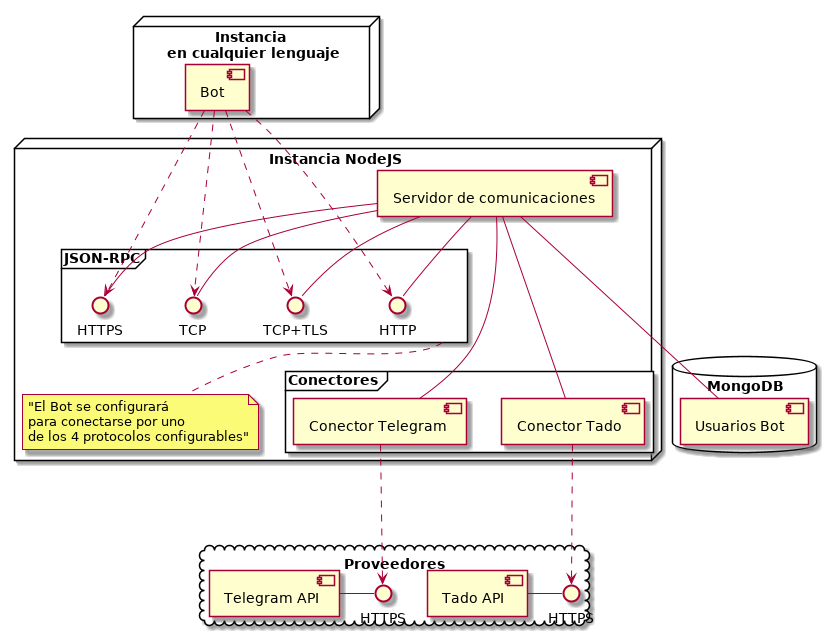
\includegraphics[width=\textwidth]{recursos/component}
\caption{Esquema de infraestructura (Diagrama de componentes)}
\label{fig:Infraestructura de nodos}
\end{figure*}

\subsection{Estructura de base de datos}

\begin{figure*}
\centering
	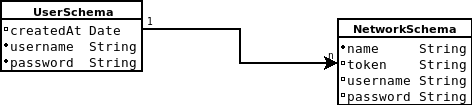
\includegraphics[width=0.65\textwidth]{recursos/schemes}
\caption{Estructura de base de datos}
\label{fig:Estructura de base de datos}
\end{figure*}

\subsection{Disposición del código}

\begin{figure*}
\centering
	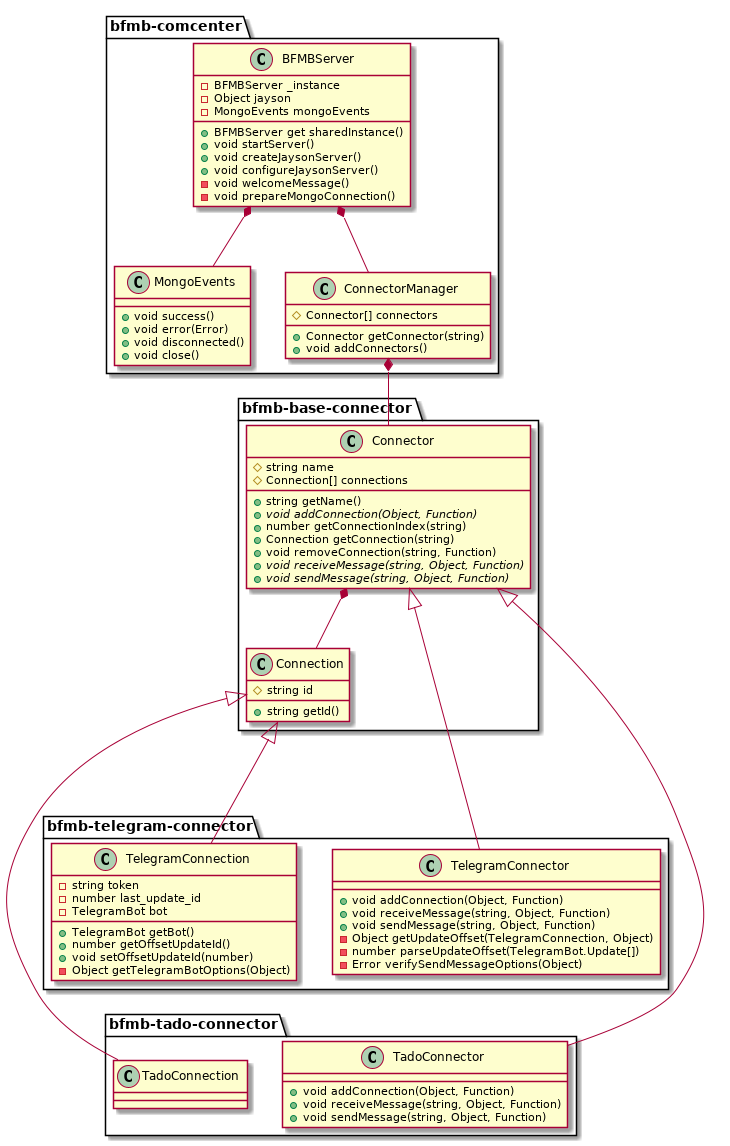
\includegraphics[width=\textwidth]{recursos/classes}
\caption{Diagrama de clases}
\label{fig:Diagrama de clases}
\end{figure*}

\section{DESARROLLO}

\subsection{Lenguaje usado en desarrollo}

El lenguaje usado para el desarrollo del software de este proyecto es Typescript, el cual vamos a hablar de él a continuación:

\subsubsection{Typescript}

Typescript es un lenguaje de programación que es un superconjunto de Javascript al que se le añade el tipado estático y la definición de objetos basados en clases. Es un proyecto de código abierto con licencia Apache 2.0 creado y mantenido por Microsoft.

\subsection{Dependencias}

\subsubsection{MongoDB}

\subsubsection{Jayson}

\subsubsection{Api de Telegram}

\subsubsection{Api de Tadoº}

\section{PRUEBAS}

\subsubsection{Mocha}

\section{MANUAL DE USUARIO}

\section{CONCLUSIONES}

\section{LÍNEAS FUTURAS}

Tras el desarrollo actual y los resultados dados, se puede ver que hay distintas líneas futuras a partir de ahora. Algunas de ellas son mejoras del software para permitir una mayor portabilidad y otras pertenecen a posibles desarrollos adicionales.

\begin{itemize}
\item Cambiar el motor de base de datos usando en el servidor de comunicaciones. 

Actualmente se usa MongoDB por conveniencia en el desarrollo del proyecto final de grado, pero sería más apropiado usar bases de datos portables como SQLite y evitar la instalación de un servidor adicional para el poco volumen de información que tiene que almacenar, aunque eso conlleve la modificación de parte del código fuente para pasar de una tecnología NoSQL a SQL.

\item Incorporar un gestor web de usuarios para el servidor de comunicaciones.

Actualmente, se están añadiendo los usuarios y configuraciones a través de un script. La incorporación de un gestor web serviría para facilitar la configuración del mencionado servidor.

\item Acoplar un motor de reconocimiento de lenguaje natural para la parte bot.

Ahora mismo, debido a problemas de tiempo de desarrollo, el bot realizado para este proyecto no procesa lenguaje natural, sino que se basa en comandos para la realización de órdenes. Se podría incorporar una implementación de ELIZA con un script personalizado para estos casos de uso. En lugar de un script psicoterapeuta, uno que reconozca frases del estilo "Pon la cocina a 23ºC" y lo asocie con la orden que debe ejecutar.

\item Cambiar la abstracción del servidor de comunicaciones a métodos de api REST (Crear, consultar, editar y eliminar). Sería la equivalencia a las acciones HTTP POST, GET, PUT y DELETE en lugar de tener una abstracción de dos métodos (\emph{receive} y \emph{send}).
\end{itemize}

\section*{ANEXOS}


%	REFERENCIAS
\newpage

\begin{thebibliography}{00}
\bibitem{CANLI} \textsc{Pérez-Diaz, D.} y \textsc{Pascual-Nieto, I.},
	\textit{Conversational Agents and Natural Language Interaction: Techniques and Effective Practices}, IGI Global, 2011 ISBN: 9781609606183
	
\bibitem{PCBEvolution} \textsc{Cerdas Mendez, D.}
	\textit{Historia de los chatbots y asistentes virtuales}, Planeta Chatbot, \url{https://planetachatbot.com/evolucion-de-los-chatbots-48ff7d670201}, [Visitado el 4/3/2019]
	
\bibitem{WeizenbaumNYT} \textsc{Markoff, J.}
	\textit{Joseph Weizenbaum, Famed Programmer, Is Dead at 85}, The New York Times, \url{https://www.nytimes.com/2008/03/13/world/europe/13weizenbaum.html}, [Visitado el 12/3/2019]
	
\bibitem{SCPhillipsTadoIEng} \textsc{Phillips, S.}
	\textit{The Tado API v2}, SCPhillips.com, \url{http://blog.scphillips.com/posts/2017/01/the-tado-api-v2/}, [Visitado el 12/3/2019]
	
\bibitem{JSONRPC} \textsc{JSON-RPC Working Group} \textit{JSON-RPC version 2.0 specification}, \url{https://www.jsonrpc.org/specification}, [Visitado el 8/4/2019]

\bibitem{CleanTechTado} \textsc{Cleantech investor} \textit{Tadoº raises \texteuro10m from Target Partners and Shortcut Ventures}, \url{https://web.archive.org/web/20140821174647/http://www.cleantechinvestor.com/portal/mainmenucomp/companiest/3258-tado/11706-tado-raises.html}, [Visitado el 17/4/2019]

\bibitem{TadoDeviceSpecs} \textsc{Tado GmbH} \textit{Technical documentation of Tado}, \url{http://www.free-instruction-manuals.com/pdf/pa_1184164.pdf}, [Visitado el 19/4/2019]

\bibitem{Tado6LoWPAN} \textsc{Jiménez Ruiz, L.} \textit{Diseño e implementación de etapa de comunicación basada en 6LoWPNA para plataforma modular de redes de sensores inalámbricas}, Archivo documental de la UPM, 2016, \url{http://oa.upm.es/43013/1/TFG_LUIS_JIMENEZ_RUIZ.pdf}, [Visitado el 19/4/2019]

\bibitem{TelegramFAQ} \textsc{Telegram} \textit{Telegram FAQ}, \url{https://telegram.org/faq}, [Visitado el 19/4/2019]

\bibitem{TelegramLogin} \textsc{Telegram} \textit{Telegram Login for Websites}, \url{https://telegram.org/blog/login}, [Visitado el 19/4/2019]

\bibitem{FrameworkJJG} \textsc{J. Gutiérrez, J.} \textit{¿Qué es un framework web?}, \url{http://www.lsi.us.es/~javierj/investigacion_ficheros/Framework.pdf}, [Visitado el 5/5/2019]
\end{thebibliography}
\end{document}

